
\glsresetall
\section{Introduction}
    As more of society becomes integrated with \gls{ml}, topics related to bias, fairness, and the formalization of \gls{ml} standards attract more attention~\cite{10.1007/978-3-030-13469-3_68, anne2018women, wang2018racial}. Thus, an effect of the growing dependency on \gls{ml} is an ever-increasing concern about the biased and unfair algorithms, \eg untrustworthy and prejudiced \gls{fr}~\cite{nagpal2019deep,snow2018}.
    


    Nowadays, \glspl{cnn} are trained on faces identified by a detection system. Specifically, for \gls{fr}, the goal is to encode faces in an N-dimensional space such that samples of the same identity are neighbors, while different persons are farther apart. Thus, we can deploy a \gls{cnn} to encode faces, and then compare via a similarity score (\ie pairs with a high enough score classified as \emph{genuine}; else, \emph{imposter}). 

\begin{figure}
    \centering
    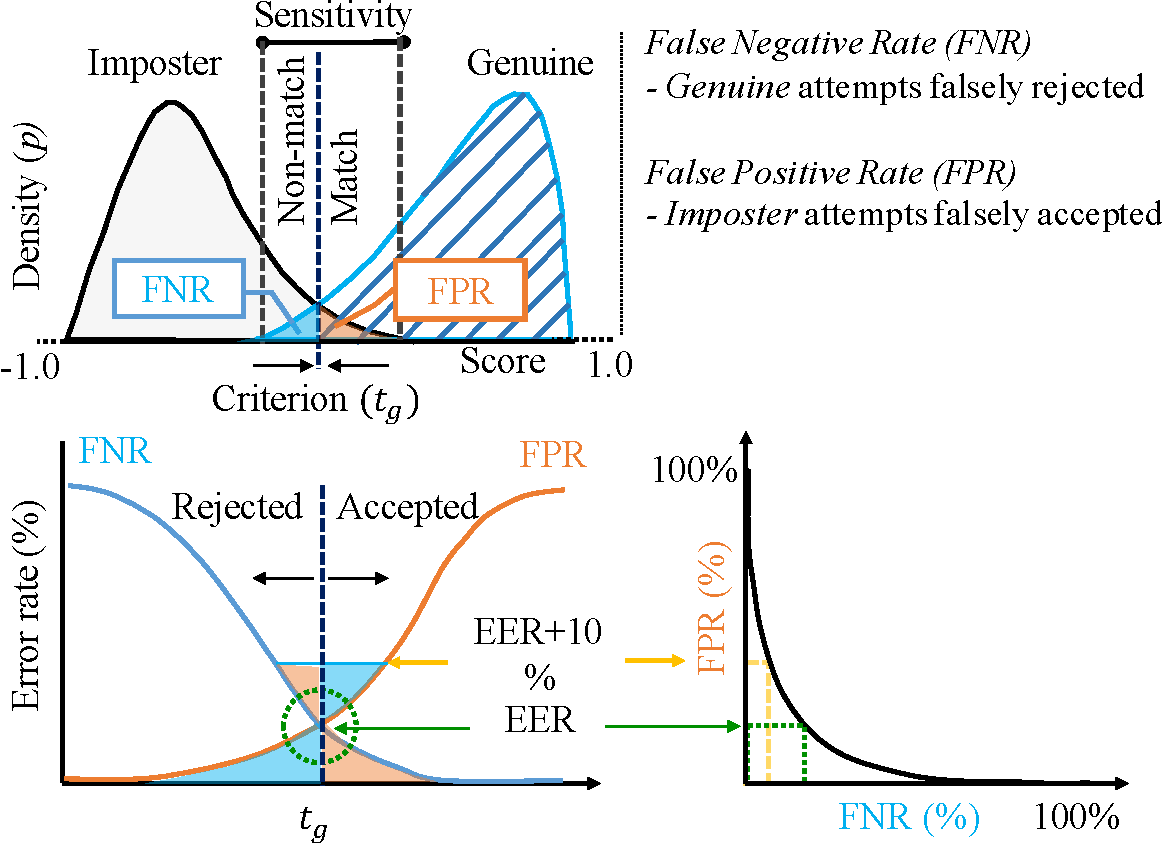
\includegraphics[width=\linewidth]{figures/fig1-crop.pdf}
    \caption{\small{\textbf{Depiction of bio-metrics.} The \gls{sdm} (\emph{top-left}) shows the sensitivity related to a single threshold $t_g$. Translated to error rate (\emph{bottom-left}), a direct trade-off between FNP and FPR. In practice, this is entirely application dependent. Specifically, the specific chose in desired FPR (\%) (\emph{bottom-right}).}}
    \label{fig:biometrics}
\end{figure}

    
Typically, a fixed threshold sets the decision boundary by which to compare scores (Fig.~\ref{fig:biometrics}). As such, features of the same identity must satisfy a criterion based on a single value~\cite{deng2019arcface, liu2017sphereface, wang2018additive, wang2018cosface}. However, we found that an individual (\ie global) threshold is a crude measure that leads to skewed errors. Furthermore, the held-out set used to determine the threshold tends to share the same distribution with the test set, favoring specific demographics that are the majority. That skew (\ie the difference in the performance of an algorithm of particular demographics) is our definition of bias. A key question is: \emph{is \gls{fr} too biased, or not?} 
    

\begin{table*}[!t]
    \centering
    \caption{\small{\textbf{Database stats and nomenclature.} \textit{Header:} Subgroup definitions. \textit{Top:} Statistics of \gls{bfw}. \textit{Bottom:} Number of pairs for each partition. Columns grouped by ethnicity and then further split by gender.}}\label{tab:ethnic-splits}
    \scalebox{.75}{
     \resizebox{\textwidth}{!}{%
    \begin{tabular}{r c c c c c c c c l}
        \toprule
        & \multicolumn{2}{c}{Asian (A)} & \multicolumn{2}{c}{Black (B)}  & \multicolumn{2}{c}{Indian (I)}& \multicolumn{2}{c}{White (W)}\\
        \cmidrule(l){2-3} \cmidrule(l){4-5} \cmidrule(l){6-7}\cmidrule(l){8-9} % spanning less than the full width of the table - you can add (r) or (l) just before the opening curly bracket to shorten the rule on the left or right side
         & Female (AF) & Male (AM) & BF & BM& IF & IM & WF & WM&Aggregated\\ % Column names row
        \midrule

       \# Faces  &  2,500&  2,500& 2,500 & 2,500& 2,500 & 2,500 & 2,500 & 2,500 &20,000 \\ % row 1
        \# Subjects & 100& 100& 100  & 100  & 100  & 100& 100 &100&800  \\ % row 2
        \# Faces / Subject  & 25 & 25    & 25 & 25 & 25  & 25  &  25 & 25 & 25\\ % row 3
        % \midrule
\specialrule{.01em}{.05em}{.05em}
            \# Positive Pairs &  30,000&  30,000& 30,000 &30,000 & 30,000 &30,000&30,000 & 30,000 &240,000 \\ % row 1
        \# Negative Pairs & 85,135&  85,232& 85,016  & 85,141  & 85,287  & 85,152& 85,223 &85,193&681,379  \\ % row 2

        \# Pairs (Total) & 115,135 & 115,232    &115016 &115,141 & 115287  & 115,152  &  115,223& 115193 & 921,379\\ % row 3
        % \midrule
        % \specialrule{.01em}{.05em}{.05em}
        % Acc$@t_g$ & 0.941 & 0.952  & 0.967 & 0.960 & 0.958 &0.962  & 0.973 & 0.981 &0.962 $\pm$0.012 \\
        % $t_o$ & 0.255 &  0.246 & 0.277 &0.242  &0.297 & 0.264& 0.233 &0.239 &0.257$\pm$0.006\\ % row 4
        
        % Acc$@t_o$ & 0.942 &0.952 &0.968 &0.961 &0.960 &0.962 & 0.974 &0.982 & 0.963 $\pm$ 0.012\\
        \bottomrule
    \end{tabular}}
    }
    \vspace{-12pt}
\end{table*}

    
    Making matters more challenging, precise definition of race and ethnicity vary from source-to-source. For example, the US Census Bureau allows an individual to self-identify race.\footnote{\scriptsize\href{https://www.census.gov/mso/www/training/pdf/race-ethnicity-onepager.pdf}{www.census.gov/mso/www/training/pdf/race-ethnicity-onepager}} Even gender, our attempt to encapsulate the complexities of the sex of a human as one of two labels. Others have addressed the oversimplified class labels by representing gender as a continuous value between 0 and 1 - rarely is a person entirely \emph{M} or \emph{F}, but most are somewhere in between~\cite{merler2019diversity}. For this work, we define subgroups as specific sub-populations with face characteristics similar to others in a region. Specifically, we focus on 8 subgroups (Fig.~\ref{fig:avg-faces}).
    
    
    The adverse effects of a global threshold are two-fold: \textbf{(1)} mappings produced by \glspl{cnn} are nonuniform. Therefore, distances between pairs of faces in different demographics vary in distribution of similarity scores (Fig~\ref{fig:detection-model}); \textbf{(2)} evaluation set is imbalanced. Subgroups that make up a majority of the population will carry most weight on the reported performance ratings. Reported results favor the common traits over the underrepresented. Demographics like gender, ethnicity, race, and age are underrepresented in most public datasets~\cite{merler2019diversity, wang2018racial}. 
    
    
    For \textbf{(1)}, we propose subgroup-specific (\ie optimal) thresholds while addressing \textbf{(2)} with a new benchmark dataset to measure bias in \gls{fr}, \gls{bfw} (Table~\ref{tab:ethnic-splits} and~\ref{tab:compared}). \gls{bfw} serves as a proxy for fair evaluations for \gls{fr} while enabling per subgroup ratings to be reported. We use \gls{bfw} to gain an understanding of the extent to which bias is present in \gls{soa} \gls{cnn}s used \gls{fr}. Then, we suggest a mechanism to mitigate problems of bias with more balanced performance ratings for different demographics. Specifically, we propose using an adaptive threshold that varies depending on the characteristics of detected facial attributes (\ie gender and ethnicity). We show an increase in accuracy with a balanced performance for different subgroups. Similarly, we show a positive effect of adjusting the similarity threshold based on the facial features of matched faces. Thus, selective use of similarity thresholds in current \gls{soa} \gls{fr} systems provides more intuition in \gls{fr} research with a method easy to adopt in practice. 
    
    
    The contributions of this work are 3-fold. (1) We built a balanced dataset as a proxy to measure verification performance per subgroup for studies of bias in \gls{fr}. (2) We revealed an unwanted bias in scores of face pairs - a bias that causes ratings to skew across demographics. For this, we showed that an adaptive threshold per subgroup balances performance (\ie the typical use of a global threshold unfavorable, which we address via optimal thresholds). (3) We surveyed humans to demonstrate bias in human perception (NIH-certified, \textit{Protect Humans in Research}).%\footnote{NIH-certified, \textit{Protect Humans in Research}.}%19-09-08}.}

